
\documentclass[foo.tex]{subfiles}
\begin{document}

\section{Galactic Properties}
\label{sec:galprops}

% fig 1
\begin{figure*}
\centering
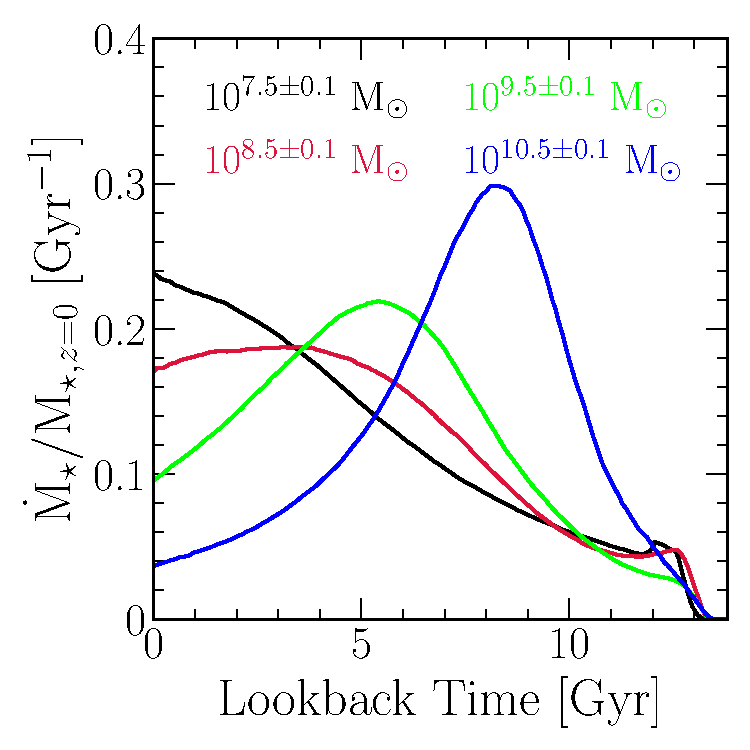
\includegraphics[scale = 0.45]{umachine_sfhs.pdf}
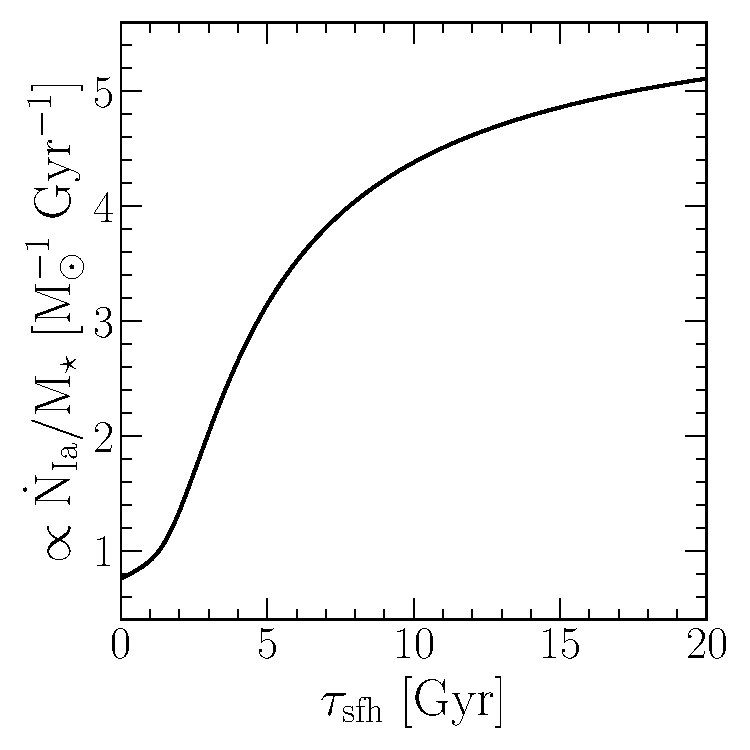
\includegraphics[scale = 0.44]{iarate_vs_tausfh.pdf}
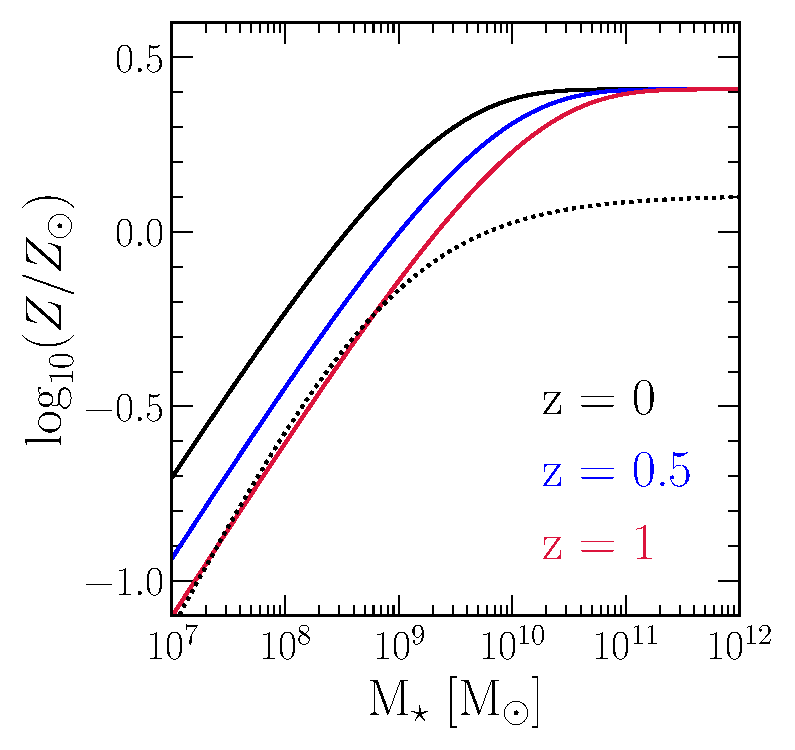
\includegraphics[scale = 0.44]{mzr.pdf}
\caption{
\textbf{Left}: The best-fit mean SFHs of the~\um~galaxies with present-day
stellar masses of $\mstar = 10^{7.5 \pm 0.1}$ (black),~$10^{8.5 \pm 0.1}$ (red),
$10^{9.5 \pm 0.1}$ (green), and $10^{10.5 \pm 0.1} \msun$ (blue) normalized by
their present-day stellar masses.
\textbf{Middle}: The specific SN Ia rate as a function of the e-folding
timescale of the SFH~$\tau_\text{sfh}$ assuming a linear-exponential time
dependence and a~$\tau^{-1}$ power-law SN Ia DTD.
\textbf{Right}: The redshift-dependent MZR reported by~\citet{Zahid2014} at
$z = 0$ (black solid),~$z = 0.5$ (blue), and~$z = 1$ (red).
For comparison, we include the~$z \approx 0$ MZR measured by
\citet[][black dotted]{Andrews2013}.
}
\label{fig:sfh_mzr}
\end{figure*}

We begin by examining how the mean galactic SFH varies with present-day stellar
mass as predicted by the~\um~semi-empirical model~\citep{Behroozi2019}.
{\color{red}
While conventional semi-analytic models forward model galaxy
formation (see, e.g., the review in~\citealt{Somerville2015a}),~\um~uses dark
matter halo properties from the~\textit{Bolshoi-Planck} and
\textit{Multi-Dark Planck 2} dark matter only simulations~\citep{Klypin2016}
to fit continuity equations to the observations.
It successfully reproduces a broad range of well-constrained observables,
including stellar mass functions, cosmic SFRs, specific SFRs, quenched
fractions, and UV luminosity functions.
}
% Using dark matter halo properties supplied by the~\textit{Bolshoi-Planck} and
% \textit{Multi-Dark Planck 2} dark matter only simulations~\citep{Klypin2016,
% RodriguezPuebla2016},~\um~follows a conventional semi-analytic model framework
% (see, e.g., the review in~\citealt{Somerville2015a}) and successfully
% reproduces a broad range of well-constrained observables, including stellar
% mass functions, cosmic SFRs, specific SFRs, quenched fractions, and UV
% luminosity functions.
While some semi-analytic models have used the extended Press-Schechter
formalism~\citep{Press1974, Bond1991} to generate halo merger trees and push
the lower stellar mass limit of their model down to~$\mstar \approx 10^7~\msun$
\citep[e.g.][]{Somerville2015b}, an advantage of~\um~is that the high mass
resolution of the~\textit{Bolshoi-Planck} and~\textit{Multi-Dark Planck 2}
simulations allows merger trees down to~$\mstar = 10^{7.2}~\msun$ to be
obtained directly from the simulations.
Conveniently, this limit is approximately the lowest mass for which there are
empirical constraints on the specific SN Ia rate from ASAS-SN~\citep{Brown2019}
and DES~\citep{Wiseman2021}%
{\color{red}%
, though one source of uncertainty is that~\um's constraints on SFHs at these
masses involve significant extrapolation.}
To relate these predictions to data from the untargeted ASAS-SN
survey~\citep{Shappee2014, Kochanek2017}, we take the full galaxy
sample from~\um, including both star forming and quenched galaxies as
well as both centrals and satellites, though centrals are the dominant
population across the full stellar mass range.
\par
In the left panel of Fig.~\ref{fig:sfh_mzr}, we show the best-fit mean SFH as a
function of lookback time in four narrow bins of present day stellar mass.
In general, low stellar mass galaxies have more extended SFHs than their
higher mass counterparts.
This effect is sufficiently strong that for stellar masses of
$\sim$$10^{7.5}~\msun$, typical SFRs are still increasing at the present day,
while~$\sim$$10^{10.5}~\msun$ galaxies experienced their fastest star formation
long ago.
\par
We adopt a DTD that scales with the age of a stellar population as~$\tau^{-1}$
starting at a delay time~$t_\text{D} = 100$ Myr as suggested by comparisons of
the cosmic SFH with the volumetric SN Ia rate as a function of redshift
(\citealp{Maoz2012a};~\citealp*{Maoz2012b};~\citealp{Graur2013, Graur2014}).
We conducted our analysis using alternative choices of the power-law
index as well as an exponential DTD with an e-folding timescale of
$\tau_\text{Ia} = 1.5$ Gyr and found similar conclusions in all cases.
We do not consider metallicity-dependent variations in the shape of the DTD
here, instead focusing on the overall normalization.
In principle, the minimum delay of the DTD could be as short as~$\sim$40 Myr if
WDs are produced by~$\lesssim$8~\msun~stars~\citep*[e.g.,][]{Hurley2000}, and
perhaps even shorter at low metallicity if the total metal content of a star
significantly impacts its lifetime~\citep[e.g.,][]{Kodama1997, Vincenzo2016}.
However, if SNe Ia require some additional time following WD formation, the
minimum delay will be longer.
Since we are interested in the first-order effects of variations in the SFH on
specific SN Ia rates, we assume a value of~$t_\text{D} = 100$ Myr.
In calculations using both~$t_\text{D} = 40$ Myr and~$t_\text{D} = 150$ Myr,
we found similar results.
\par
% \par
% Although the details of the SN Ia DTD have been a topic of active inquiry for
% some time~\citep[e.g.][]{Greggio2005, Strolger2020, Freundlich2021},
% comparisons of the cosmic SFH~\citep[e.g.][]{Hopkins2006, Davies2016, Madau2014,
% Madau2017, Driver2018} with the volumetric SN Ia rate as a function of redshift
% suggest that the cosmic DTD is broadly consistent with a~$\tau^{-1}$ power-law
% (\citealp{Maoz2012a};~\citealp*{Maoz2012b};~\citealp{Graur2013, Graur2014}).
% A DTD of approximately this form is also expected under the double-degenerate
% scenario given population synthesis models of binary white dwarfs and the loss
% of angular momentum due to graviational wave emission (e.g.
% \citealp{Mennekens2010};~\citealp*{Maoz2014}).
% We therefore adopt this parametrization in this paper, though we have
% reconducted our analysis using an exponential DTD with a timescale of
% $\tau_\text{Ia} = 1.5$ Gyr and found similar results.
% We do not consider metallicity-dependent variations in the shape of the DTD
% here, instead focusing on the overall normalization.
% \par
% In principle, the minimum delay time of the DTD could be as short as~$\sim$40
% Myr if WDs are produced by~$\lesssim 8~\msun$ stars~\citep*[e.g.][]{Hurley2000},
% and perhaps even shorter at low metallicity if the total metal content of a
% star significantly impacts its lifetime as in, e.g.,~\citet{Kodama1997} and
% \citet{Vincenzo2016}.
% However, if SNe Ia require some additional time following WD formation, the
% minimum delay will be longer.
% Since we are interested in demonstratin the first-order effects of variations
% in SFHs on specific SN Ia rates, we assume a value of~$t_\text{D} = 100$ Myr.
% We have also reproduced the results of this paper with both~$t_\text{D} = 40$
% Myr and~$t_\text{D} = 150$ Myr and found similar results in both cases.
% \par
For an SFH~$\dot{M}_\star$ and DTD~$R_\text{Ia}$ as functions of lookback time
$\tau$, the specific SN Ia rate at a stellar mass~$\mstar$ is
\begin{equation}
\frac{\dot{N}_\text{Ia}(M_\star | \gamma)}{M_\star} \propto Z(M_\star)^\gamma
\ddfrac{
	\int_0^{T - t_\text{D}}\dot{M}_\star(\tau | M_\star) R_\text{Ia}(\tau) d\tau
}{
	\int_0^T \dot{M}_\star(\tau | M_\star) d\tau
}
\label{eq:specia}
\end{equation}
where~$T = 13.2$ Gyr is the time elapsed between the onset of star formation
and the present day.
To investigate the effects of metallicity, we add a power-law metallicity
scaling~$Z(\mstar)^\gamma$ where~$Z$ is given by the MZR.
{\color{red}
In detail, the WDs producing SNe Ia come from stellar populations with a
distribution of metallicities, and therefore a more accurate parametrization
would marginalize~$Z(M_\star)^\gamma$ over each galaxy's enrichment history.
The inferred rates would be higher if one were to account for this effect, but
the event rate in low-mass field galaxies should be dominated by young stellar
populations anyway due to their tendency to form at low redshift combined with
the steepness of the SN Ia DTD.
Accounting for distributions in metallicity can be addressed by either
including an MZR that evolves with redshift inside the integral or folding in
some model of galactic chemical evolution (GCE; see,
e.g.,~\S~\ref{sec:gce} below or the review by~\citealp{Matteucci2021}).
}
We are only interested in the scaling of the rates with~\mstar, so we normalize
all rates to unity at~$\mstar = 10^{10}~\msun$ following~\citet{Brown2019}.
Although the denominator of equation~\refp{eq:specia} in detail should depend
on mass loss from stars as they eject their envelopes, this is an approximately
constant term which can safely be neglected in the interest of computing
relative rates ($\approx$40\% for a~\citealt{Kroupa2001} IMF; see discussion
in~\S\S~2.2 and 3.7 of~\citealt*{Weinberg2017}).
\par
To qualitatively illustrate how the specific SN Ia rate scales with the
timescale over which star formation occurs, we consider the simple example of a
linear-exponential
parametrization~$\dot{M}_\star \propto te^{-t/\tau_\text{sfh}}$ where
$t = T - \tau$.
The middle panel of Fig.~\ref{fig:sfh_mzr} shows equation~\refp{eq:specia} as
a function of the e-folding timescale~$\tau_\text{sfh}$ assuming~$\gamma = 0$.
The specific SN Ia rate is lowest in the limiting case of a single episode of
star formation (i.e.,~$\tau_\text{sfh} \rightarrow 0$), rises steeply until
$\tau_\text{sfh} \approx 10$ Gyr, and then flattens once
$\tau_\text{sfh} \gtrsim T$.
A higher specific SN Ia rate as observed in dwarf galaxies is therefore a
natural consequence of their more extended SFHs, though we demonstrate below
that this effect accounts for only a factor of~$\sim$2 increase in the rate
between~$10^{7.2}$ and~$10^{10} \msun$.
% \par
% Not only do dwarf galaxies have more extended SFHs, but the empirical MZR
% indicates that they also have a lower metal content~\citep{Tremonti2004,
% Gallazzi2005, Zahid2011, Kirby2013}.
% At low metallicities, there are multiple effects which could increase the SN Ia
% rate.
% At fixed initial mass, low metallicity stars leave behind more massive WDs due
% to weaker winds and consequently enhanced core growth during the AGB phase
% \citep{Umeda1999, Willson2000, Marigo2007, Meng2008, Zhao2012, Kalirai2014}.
% This effect could make it easier for a WD to reach the Chandrasekhar mass and
% explode (see discussion in~\citealt{Kistler2013}).
% Additionally, the stellar close binary fraction is known to increase from
% $\sim$10\% at~$\sim$3 times the metallicity of the sun~$Z_\odot$ to~$\sim$40\%
% at~$\sim0.1 Z_\odot$~\citep{Moe2019}.
% Consequently, dwarf galaxies should have more potential SN Ia progenitors per
% unit mass of star formation due to more massive WDs and a higher close binary
% fraction.
\par
The right panel of Fig.~\ref{fig:sfh_mzr} shows the MZR parametrized by
\citet[][see their equation 5]{Zahid2014}\footnote{
	We have transformed from their~$\log_{10}\text{(O/H)}$ measurements to the
	logarithmic abundance relative to the Sun~$\log_{10}(Z / Z_\odot)$ assuming
	the Solar oxygen abundance derived by~\citet{Asplund2009}.
} at redshifts~$z = 0$, 0.5 and 1 in comparison to the~\citet{Andrews2013}
parametrization at~$z = 0$.
Although~\um~allows us to investigate these effects at stellar masses as low as
$10^{7.2}~\msun$, the~\citet{Zahid2014} measurements are available only for
$\mstar \approx 10^9 - 10^{11}~\msun$ galaxies.
\citet{Andrews2013} used stacked spectra from the Sloan Digital Sky Survey
\citep[SDSS;][]{York2000} to obtain direct measurements of the oxygen abundance
in bins of stellar mass extending as low as~$\sim$$10^{7.4}~\msun$.
Relative to~\citet{Zahid2014}, the~\citet{Andrews2013} parametrization has a
lower plateau but otherwise a similar slope and turnover mass.
Because we simply normalize the rates to unity at~$\mstar = 10^{10}~\msun$,
only the shape of the MZR matters, and we find similar results using both
parametrizations.
{\color{red}
\um~includes the parametrization of metallicities as a
function of stellar mass and redshift from~\citet{Maiolino2008}, which is
similar in shape to~\citet{Andrews2013} and~\citet{Zahid2014}.
}%
In order to estimate SN Ia rates at redshifts of~$z = 0.5$ and~$z = 1$,
we use the redshift-dependent~\citet{Zahid2014} formalism
in~\S~\ref{sec:predictions}.
% \par
{\color{red}
Although these MZRs are similarly shaped, there are others in the literature
that are different, particularly at the low-mass end where the measurements are
more challenging (see, e.g., the review by~\citealt*{Kewley2019}).
}
\par
Given a present-day stellar mass, we compute its SFH as a function of
lookback time by interpolating between the stellar mass and snapshot times
included in the~\um~predictions.
We then compute the specific SN Ia rate according to equation~\refp{eq:specia}
given the implied SFH and and a~$\tau^{-1}$ DTD, amplifying the rate by a
factor of~$Z^\gamma$ where the metallicity~$Z$ is computed from the
\citet{Zahid2014} MZR.
Because these calculations are simply using the~\um~SFHs,
{\color{red} our predictions}
are unaffected by the SMF dependence of the observational estimates (i.e.,
Eq.~\ref{eq:specia} can simply be divided by~$\mstar$ as opposed to an integral
over the SMF).
{\color{red}
However, the~\um~SFHs are still dependent on the~\citet{Baldry2012} SMF,
because they use this form as an empirical constraint at~$z = 0$.
Comparing our predictions to scalings of the SN Ia rate with masses
derived from a different SMF would require updated SFHs.
}
\par
{\color{red}
The~\textit{stellar} MZR~\citep[e.g.,][]{Gallazzi2005,
Kirby2013, Simon2019} is perhaps a better relation to use than the gas-phase
MZR since the stellar populations produce the SN events.
However, given the uncertainties involved, the gas-phase measurements should be
accurate enough for a first investigation into possible origins of metallicity
dependent SN Ia rates.
While~\citeauthor{Moe2019}'s~\citeyearpar{Moe2019} metallicity dependence of
the close binary fraction is based on stellar Fe abundances, we use gas-phase
O abundances since this observable is the primary focus of population studies
of galaxy metallicities in terms of both models and measurements.
While the O and Fe abundances of stellar populations are correlated, the
relationship between the two is not linear due to the evolving contributions of
massive stars and SNe Ia (see, e.g.,~\S~\ref{sec:gce}).
% We elect not to contend with the question of which metallicity matters
% since this connection between binarity, metallicity and SN Ia rates is
% relatively new in the literature.
\par
Morevoer, binarity appears to depend on both [Fe/H] and [$\alpha$/Fe]
\citep{Mazzola2020}.
The underlying multiplicity measurements are also challenging~\citep{Moe2017,
Offner2022} but will improve in the coming years thanks to the expansion of
available data (e.g., SDSS-V;~\citealp{Kollmeier2017}).
Lastly, changes in SN rates will impact the feedback into the ISM, and by
extension the SFH, so the post-processing prescription of
equation~\refp{eq:specia} is somewhat oversimplified~\citep{Gandhi2022}.
Nonetheless, it should suffice for understanding the first-order effects of
metallicity-dependent SN Ia rates.
}
% \par
% {\color{red}
% We note that the~\textit{stellar} MZR~\citep[e.g.,][]{Gallazzi2005, Kirby2013,
% Simon2019} is perhaps a better relation to use than the gas-phase MZR for
% relating mass to metallicity since the stellar populations produce the SN
% events.
% However, we elect not to contend with the question of which metallicity matters
% as the connection between binarity, metallicity, and SN rates is relatively new
% in the literature, and the measurements carry substantial uncertainties.
% Nonetheless, it is noteworthy that our MZR uses O as its tracer while
% \citeauthor{Moe2019}'s~\citeyearpar{Moe2019} multiplicity measurements use Fe.
% To add to the complication, there are other MZRs in the literature that have
% different shapes at the low-mass end than~\citet{Andrews2013}
% and~\citet{Zahid2014} (see, e.g., the review by~\citealp{Kewley2019}).
% Binarity also appears to be a function of both [Fe/H] and [$\alpha$/Fe]
% \citep{Mazzola2020}, and the measurements themselves are rather challenging
% (see, e.g.,~\citealp{Moe2017} and the recent review by~\citealp{Offner2022}).
% Lastly, changes in SN rates should necessarily impact the feedback deposited
% into the ISM and subsequently impact the SFH, so the post-processing
% prescription of equation~\refp{eq:specia} is somewhat oversimplified
% \citep{Gandhi2022}, though it should suffice for understanding the first-order
% effects.
% }


% Further investigations of multiplicity as a function of metallicity and more
% reliable characterizations of the MZR are required to pin down the connection
% between metallicity and SN rates across the galaxy mass spectrum.




% While the observationally inferred scaling with stellar mass is significantly
% dependent upon the assumed SMF~\citep{Gandhi2022}, we emphasize that this
% theoretical approach is independent of the SMF because we are computing the
% rates using the mean SFH at a given stellar mass as opposed to from a survey
% where rates within individual galaxies are not feasible to measure.
% In the right panel of Fig.~\ref{fig:sfh_mzr} we plot the MZR at a selection of
% redshifts as parametrized by
% \citet[][see their equation 5]{Zahid2014}.\footnote{
% 	We have transformed from their~$\log_{10}\text{(O/H)}$ measurements to the
% 	logarithmic abundance relative to the sun~$\log_{10}(Z / Z_\odot)$ assuming
% 	the solar oxygen abundance derived by~\citet{Asplund2009}.
% }
% Although~\um~allows us to investigate these effects at stellar masses as low as
% $10^{7.2}~\msun$,~\citet{Zahid2014} present measurements only for the
% $\mstar \approx 10^9 - 10^{11}~\msun$ range.
% We have therefore reconducted our analysis at~$z = 0$ using the parametric form
% of~\citet{Andrews2013}.
% They use stacked spectra from the seventh data release of the Sloan Digital
% Sky Survey~\citep[SDSS;][]{York2000, Abazajian2009, Abdorrouf2022} to increase
% the signal-to-noise of the weak [OII] and [OIII] auroral lines at 7320, 7330
% and 4363~\AA~to obtain direct measurements of the electron temperatures and
% abundances in bins of stellar mass extended as low as~$\sim 10^{7.4}~\msun$.
% We show the~\citet{Andrews2013} MZR in comparison to the~\citet{Zahid2014} form
% in the right panel of Fig.~\ref{fig:sfh_mzr}.
% The~\citet{Andrews2013} parametrization has a lower plateau but otherwise a
% similar slope and turnover mass.
% Although neither~\citet{Andrews2013} nor~\citet{Zahid2014} measure the MZR
% above~$10^{11}~\msun$, both suggest that these galaxies should be on the
% plateau anyway.
% We find similar results in~\S~\ref{sec:predictions} below using both
% parametrizations because, following~\citet{Brown2019} and~\citet{Gandhi2022},
% we quantify the specific SN Ia rate as a function of stellar mass normalized to
% 1 at~$10^{10}~\msun$.
% Therefore, the normalization of the MZR is irrelevant and what determines the
% mass dependence in our calculations is the metallicity relative to that of
% a~$10^{10}~\msun$ galaxy.
% In the interest of exploring SN Ia rates at redshifts of~$z = 0.5$ and~$z = 1$,
% we retain the~\citet{Zahid2014} formalism in~\S\S~\ref{sec:predictions}
% and~\ref{sec:diagnostics} below.

\end{document}
